\section{Tactical combat - Battlescape}

So this is where all the fun happens ;) It is here that your former choices have to proof their worth as well as you will have to prove your commanding skills.
The goal of every tactical combat is quite simple: kill all those evil aliens with as few civilian (and of cause squad) looses as possible. In order to achieve this you will have to find a good balance between caution and fast proceedings. You don't want to watch all innocents die like flies just because your soldiers are afraid of the enemy.
In the course of the game you will see a wide range of settings and environments, but no matter how bad things may look like, there a some quite powerful tools at you hand to get rid of them. If you have some experience with (turn-based) tactical combat games you should find some redundant elements - and of cause you will if you ever played any other UFO before. Nevertheless you should take a short overview over the interface so you make sure you don't miss any important feature. To change the view within battlescape you may use either cursor buttons or \keybinding{WASD}. Please be aware that its also possible to change the pitch of the camera. (\keybinding{R} and \keybinding{F} by default)
There are two alternative interfaces available right now, offering identical functions of cause. In the following we will discuss bot of them. You may switch between them as often as you want until you feel familiar with one of them (options $\hookrightarrow$ game).
While the first one is heavily inspired by the classic HUD the second one (althud) tries to utilise modern techniques to achieve cleaner optics.

\subsection{Buttons - HUD}
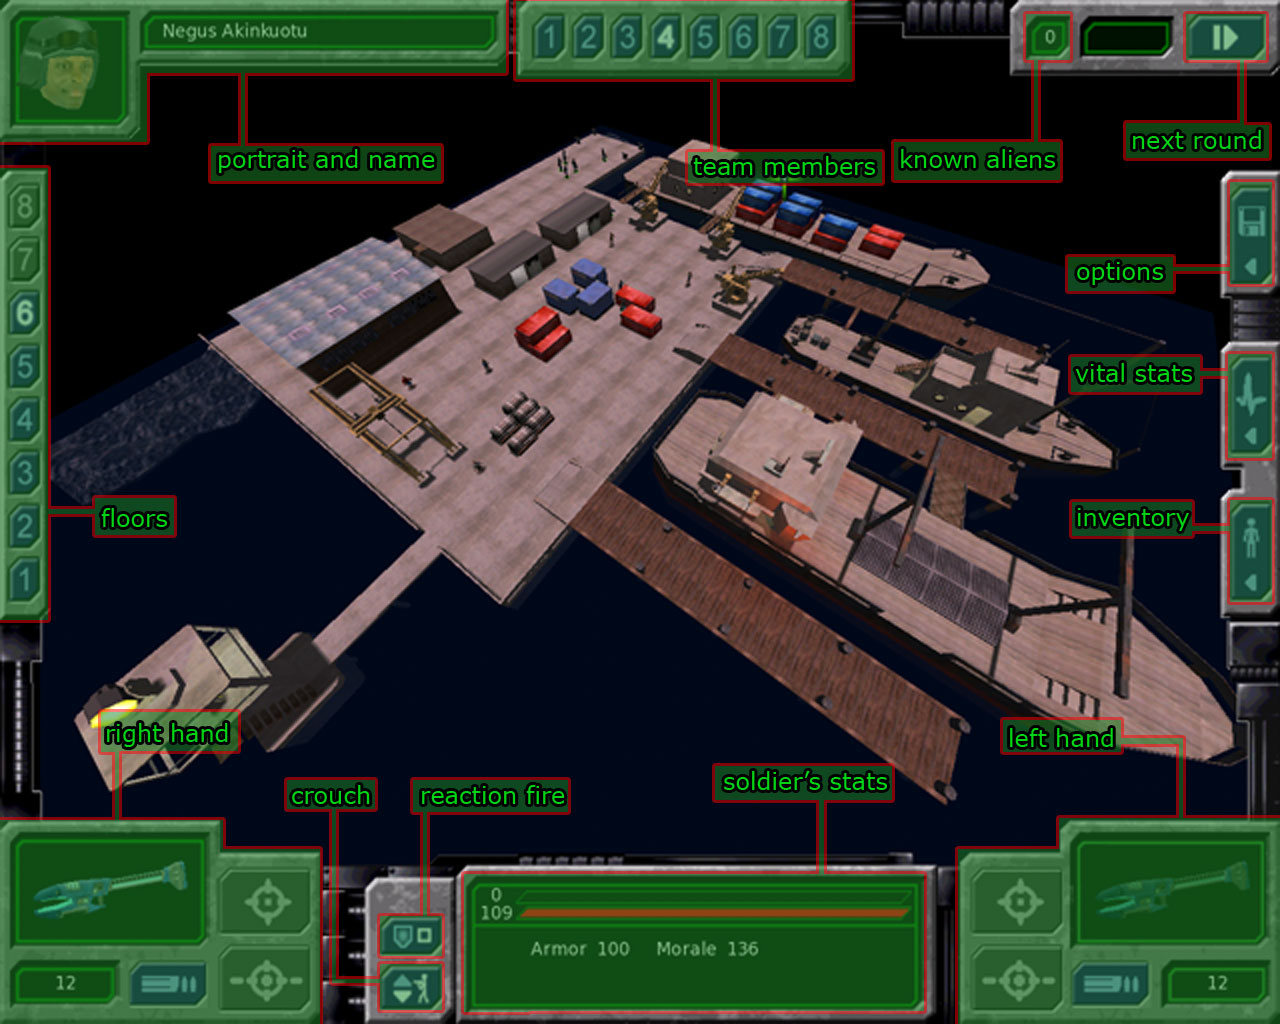
\includegraphics[width=\textwidth]{images/HUD_final.jpg}
\subsubsection{Floors}
Here you can change the ``ground-level'' or floor shown in the tactical view. Besides its obvious use in order to move you soldiers between different floor-levels it's also helpful to get an general overview. So it's always a smart move to switch between all levels at the beginning of each mission so you won't miss the ``hidden'' cellar or rooftop.
\subsubsection{Portrait and name}
This is more for aesthetic reasons, so no big actions are bound to this. (But of cause - as usual- suggestions are welcome)
\subsubsection{Team-members}
There is where you can switch between you soldiers (alternatively use keybindings: 1 to 8 or just left-click on their model). In case one (or more *G*) of your devoted fighters lost their live fighting the evil his button will become grey.
\subsubsection{Known aliens}
This states the number of aliens all your squad member have discovered this round. By clicking on it you may switch through all of them.
\subsubsection{Next round}
Hmm... so what do you suspect this one does? Exactly!
\subsubsection{Options}
Opens the ``Options''-menu where you may vary several video/sound-settings as well as abort or retry current missions. Be aware that it's not possible nor intended to save a ongoing mission. If you abort the current mission, all your soldiers will be lost.
\subsubsection{Vital stats}
This is where you find more detailed information about health, moral and psi-power of your soldier.
\subsubsection{Inventory}
Opens the inventory of the selected soldier. This is where you can change weapons, pick up/drop items or just take a look at your great heroes.
\subsubsection{Soldiers stats}
This is a summery of all general information you need to use your soldier most efficiently. Its content interacts with your mouse action, but should be quite self-explaining. Not only you will find health and remaining TUs (we will deal with TUs in the following section) here but also it will give you the amount your currently selected shooting-mode will consume as well as some other info's like current armor and moral.
\subsubsection{Reaction fire}
This button enables ``reaction fire'', a central concept of every tactical combat. We will deal with it in the following chapter. For now you should just remember that it is here where you turn it on and off.
\subsubsection{Crouch}
As one might guess, this button will make your soldier kneel down (and by doing so reducing the danger of being hit by enemy fire) or if he already does make him stand up. Please notice that a soldier that kneels down can still move forward as if he would stand upright, but it takes him 1 additional time unit per square to do so.
\subsubsection{Right/left-hand}
Those two fields are completely identical besides the fact the left hand one is active only if you actually wear two one-handed items/weapons. If you have a two-handed item/weapon equipped the left-hand field will be inactive. Because each of the two fields consist of several important buttons itself we will discuss them a bit more detailed. Please take a look at the following image.\\
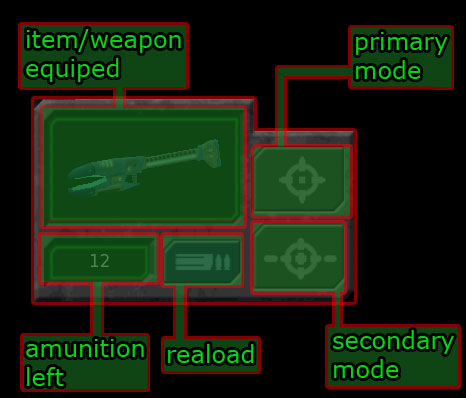
\includegraphics[width=6cm]{images/HUD_detail_final.jpg}
%as float ?!
%transparent background ?! ->going to be re-worked soon
\subsubsection{Item/weapon}
Gives a picture of the currently equipped item/weapon. This turns red in case you can't use the weapon, for example because you don't know the tech or don't have any ammunition left.
\subsubsection{Primary-mode}
Activates primary-mode for this item. In case of weapons this is usually (but not always!) a fast but less accurate / powerful shoot. For details see weapon description.
\subparagraph{Secondary-mode}
Activates secondary-mode for this item. In case of weapons this is usually (but again, not always!) a more TU-consuming but also more accurate / powerful shoot. Please notice that in case the item supports only one mode (like stun rod) both modes are identical.
\subsubsection{Reload}
Reloads currently equipped weapon, if ammunition is left in the inventory.
\subparagraph{Ammunition left}
Shows the ammunition left in your weapon. Please notice that some shooting-modes (also some of the one-shoot ones) require more than one ``bullet'' here.

\subsection{Buttons - altHUD}

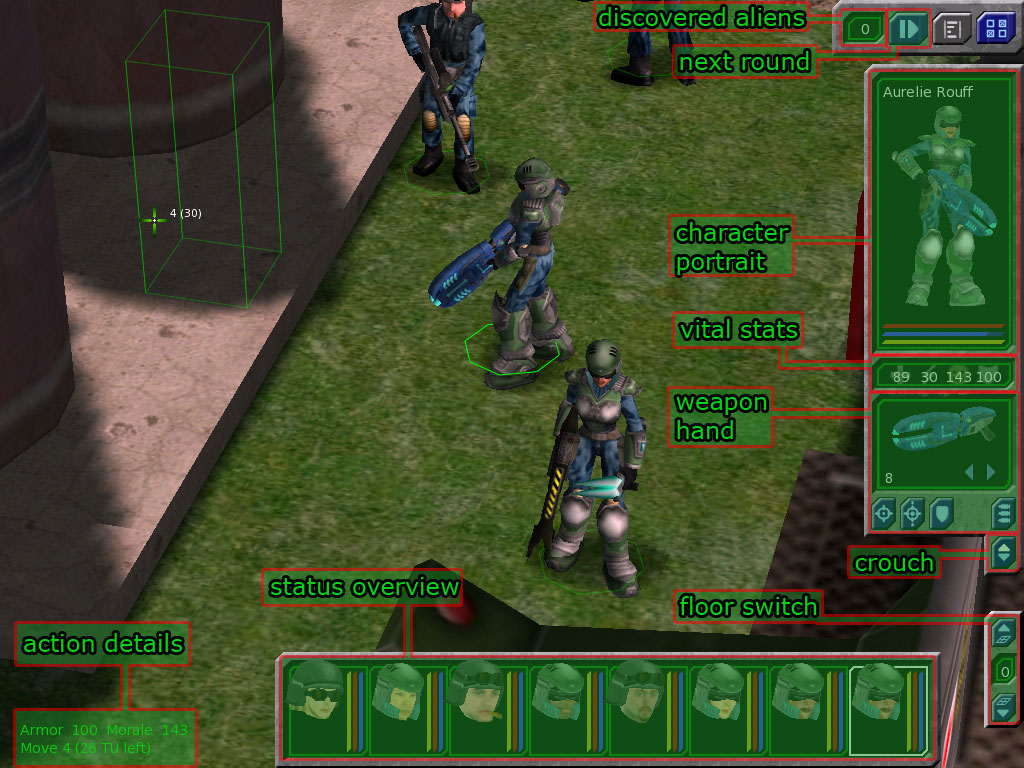
\includegraphics[width=\textwidth]{images/altHUD_final.jpg}\\

\subsubsection{Discovered aliens}
This states the number of aliens all your squad member have discovered this round. By clicking on it you may switch through all of them.
\subsubsection{Next round}
Hmm\ldots so what do you suspect this one does? Exactly!
\subsubsection{Options}
Opens the ``Options''-menu where you may vary several video/sound-settings as well as aboard or retry current missions. Be aware that it's not possible nor intended to save a ongoing mission.
\subsubsection{Character portrait}
Besides giving you the chance to admire your well dressed and equipped soldiers clicking on a soldiers portrait opens up his or her inventory.
\subsubsection{Vital stats}
This is where you find more detailed information about (from left to right) health, remaining TUs, moral and armor of your soldier.
\subsubsection{Action details}
Here some more details on your current action are displayed. If you are about to move your soldier this means you will be shown the required TU costs as well as how many will be left (if any) at the end of this action. In case you have selected one of the two firemodes you will be informed about the TU costs and the approximate probability to hit the target. Hint: Even with an 100\% chance it is still possible (but very unlikely) that your soldier failed to hit the target for unforeseeable  reasons.
\subsubsection{Crouch}
As one might guess, this button will make your soldier kneel down (and by doing so reducing the danger of being hit by enemy fire) or if he already does make him stand up. Please notice that a soldier that kneels down can still move forward as if he would stand upright, but it takes him 1 additional time unit per square to do so.
\subsubsection{Floor switch}
Here you can change the ``ground-level'' or floor shown in the tactical view. Besides its obvious use in order to move you soldiers between different floor-levels it's also helpful to get an general overview. So it's always a smart move to switch between all levels at the beginning of each mission so you won't miss the ``hidden'' cellar or rooftop.
\subsubsection{Status overview}
There is where you can switch between you soldiers (alternatively use keybindings: \keybinding{1} to \keybinding{8} or just left-click on their model). In case one (or more *G*) of your devoted fighters lost their life fighting the evil, his button disappears. Three different ??? give you an fast overview over your teams vital statistics. Red representing health points, yellow moral and blue the amount of remaining time units.
\subsubsection{Weapon hand}
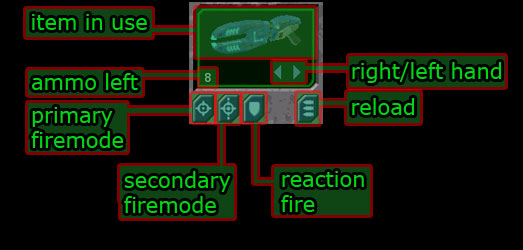
\includegraphics[width=6cm]{images/altHUD_detail_final.jpg}

\subsubsection{Weapon in use}
Gives a picture of the currently equipped item/weapon. This turns red in case you can't use the weapon, for example because you don't know the tech or don't have any ammunition left.
\subsubsection{Ammo left}
Shows the ammunition left in your weapon. Please notice that some shooting-modes (also some of the single shot ones) require more than one ``bullet'' here.
\subsubsection{Primary firemode}
Activates primary-mode for this item. In case of weapons this is usually (but not always!) a fast but less accurate / powerful shoot. For Details see weapon description.
\subsubsection{Secondary firemode}
Activates secondary-mode for this item. In case of weapons this is usually (but again, not always!) a more TU-consuming but also more accurate / powerful shot. Please notice that in case the item supports only one mode (like stun rod) both modes are identical.
\subsubsection{Reaction fire}
This button enables ``reaction fire'', a central concept of every tactical combat. We will deal with it in the following chapter. For now you should just remember that it is here where you turn it on and off.
\subsubsection{Reload}
Reloads currently equipped weapon, if ammunition is left in the inventory (consumes TUs).
\subsubsection{Right/left hand}
Switches between the left and right hands item (in case the soldier carries two one handed items).

